\documentclass[sigconf,nonacm]{acmart}
\usepackage{booktabs}
\usepackage{graphicx}
\usepackage{microtype}

% Micro-spacing adjustments for floats to guarantee strict 2-page fit
\setlength{\textfloatsep}{5pt plus 1pt minus 1pt}
\setlength{\floatsep}{5pt plus 1pt minus 1pt}
\setlength{\intextsep}{5pt plus 1pt minus 1pt}
\setlength{\abovecaptionskip}{3pt plus 1pt minus 1pt}
\setlength{\belowcaptionskip}{2pt plus 1pt minus 1pt}

\title{The Hidden Cost of Parity: Statistical Audit and Global Net Economic Impact of Parity-Aware BPE}

\author{João Vitor de Carvalho Silva}
\affiliation{}
\email{joaovitorcarvalho@dcc.ufmg.br}

\author{Lucas de Oliveira Ferreira}
\affiliation{}
\email{lucasdeoliveira@dcc.ufmg.br}

\author{Mariana Assis Ramos}
\affiliation{}
\email{mariana.assis@dcc.ufmg.br}

\begin{abstract}
Parity-Aware Byte-Pair Encoding (PA-BPE) aims to mitigate cross-lingual inequities by reallocating subword merges to maximize the compression of disadvantaged languages, claiming up to $89\%$ lower tokenization inequality (gini) without much degradation. We conduct an technical and economic audit combining the official codebase with Miller's (2024) super-population framework. First, question-level pairing and cross-lingual clustered standard errors reveal that small performance variations are statistically indistinguishable from zero ($p > 0.05$ across all 22 languages; and clustering inflates global uncertainty by $2.80\times$). Second, statistical power analysis can demonstrate that $100\%$ of benchmarks aren't able to detect a $1\%$ or $2\%$ regression (mean MDE $\pm 9.88\%$), while the algorithm induces much over-segmentation ($+62\%$ to $+330\%$) in code, arithmetic, and structured JSON. Third, crossing token counts on FLORES-200 with empirical web traffic distributions (W3Techs) and commercial API pricing (GPT-4o, Claude 3.5, Llama 3.1) uncovers an asymmetric ``English Tax'' ($+\$81.03$/1M requests on GPT-4o) that minimizes multilingual savings ($-\$39.87$), yielding a net commercial surcharge breaking even only when English traffic drops below $35.5\%$.
\end{abstract}

\begin{document}
\maketitle

\section{Introduction}
\label{sec:intro}

Subword tokenization via Byte-Pair Encoding (BPE) introduces big cross-lingual inequities in Large language Models (LLMs)~\cite{petrov2023language,ahia2023all}. Pre-training frequency biases allocate disproportional merges to English ($\sim$4.0 chars/token), forcing low-resource and non-Latin scripts (e.g., Tamil, Persian) to pay a big ``token tax'' in latency and API costs ($\le$1.5 chars/token)~\cite{ahia2023all,nllb2022no}.

To mitigate this, Foroutan et al.~\cite{foroutan2026parity} proposed \textit{Parity-Aware BPE} (PA-BPE). By replacing greedy global merging with a fair-max criterion targeting the worst-compressed, they claim an $89\%$ Gini inequality reduction without downstream degradation, at minor English compression cost.

In this group project, we present an independent empirical and economic analysis of PA-BPE, combining its codebase~\cite{foroutan2026parity} with the super-population framework of Miller~\cite{miller2024adding}:
\begin{itemize}
    \item \textbf{Downstream Significance (Sec.~\ref{sec:results_significance}):} Accuracy differences between standard and fair tokenizers are statistically indistinguishable from zero ($p > 0.05$ across all 22 languages) when evaluated with proper pairing and clustering.
    \item \textbf{Power \& Failure Modes (Sec.~\ref{sec:power_and_failures}):} Evaluation benchmarks are, in general, underpowered ($\mathrm{MDE} \pm 9.9\%$), while PA-BPE fragments code, math, and structured JSON ($+62\%$ to $+330\%$).
    \item \textbf{Global API Economics (Sec.~\ref{sec:financial_impact}):} On real web traffic (W3Techs), the ``English Tax'' decisively outweighs multilingual savings, generating a net commercial loss unless English traffic drops below $35.5\%$.
\end{itemize}

\section{Background \& Evaluation Paradox}
\label{sec:background}

While classical BPE greedily merges the globally most frequent pairs $\sum_l \mathrm{Count}_l(p_1, p_2)$, PA-BPE's \textit{fair-max} reallocates merges to the language with the minimum compression ratio $\mathrm{CR}_l = |\mathcal{C}_l|_{\mathrm{chars}} / |\mathcal{C}_l|_{\mathrm{tokens}}$. 

However, evaluating fairness via isolated benchmark standard errors ($\hat{\mu} \pm \mathrm{SE}$) introduces a lot of validity flaws: as it omits positive question-level pairing covariance ($\rho > 0$) and treats parallel translated instances of identical questions across languages as independent (this violates the Central Limit Theorem~\cite{miller2024adding}).

\section{Methodology}

\subsection{Statistical Audit Framework (Miller, 2024)}
\label{sec:stat_methodology}

To audit claimed downstream parity~\cite{foroutan2026parity}, we implemented Miller's super-population framework~\cite{miller2024adding}. Because model $A$ (PA-BPE) and baseline $B$ (Classical BPE) are evaluated on identical prompts, analyzing paired differences $d_i = s_{A,i} - s_{B,i}$ isolates model variance (Miller Eq.~7):
\begin{equation}
\mathrm{SE}_{A-B,\mathrm{paired}} = \sqrt{\mathrm{SE}_A^2 + \mathrm{SE}_B^2 - 2\rho\,\mathrm{SE}_A\mathrm{SE}_B}.
\label{eq:paired_se}
\end{equation}
Crucially, multilingual benchmarks translate identical questions $c \in \{1,\dots,C\}$ across languages. Treating them as independent violates the Central Limit Theorem. Due to that, we apply the paired, cluster-adjusted standard error (Miller Eq.~8):
\begin{equation}
\mathrm{SE}_{A-B,\mathrm{clustered}} = \frac{1}{n}\left(\sum_{c=1}^{C}\sum_{i \in c}\sum_{j \in c}(d_{i,c} - \bar{d})(d_{j,c} - \bar{d})\right)^{\!1/2}\!\!,
\label{eq:clustered_se}
\end{equation}
yielding cluster-robust 95\% confidence intervals $\bar{d} \pm 1.96\,\mathrm{SE}_{\mathrm{clustered}}$.

\begin{figure}[t]
    \centering
    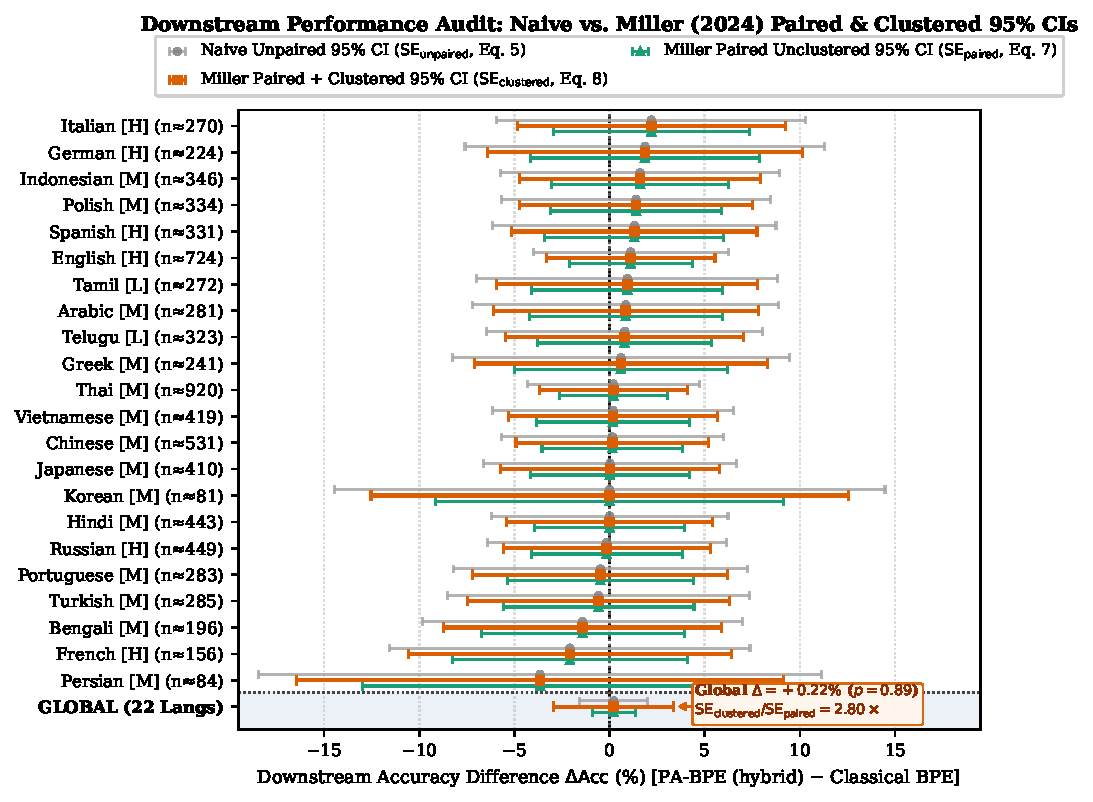
\includegraphics[width=0.98\columnwidth]{figures/fig1_forest_plot.pdf}
    \caption{Downstream $\Delta\mathrm{Acc}$ (\textbf{PA-BPE hybrid $-$ Classical BPE}) across 22 languages. Clustering inflates global uncertainty by $\mathbf{2.80\times}$; all 22 languages cross zero at 95\% CI.}
    \label{fig:forest_plot}
    \vspace{-0.6em}
\end{figure}

\subsection{Downstream Significance Audit Results}
\label{sec:results_significance}

Figure~\ref{fig:forest_plot} presents our audit of Table~2 from~\cite{foroutan2026parity}. Inverting Bernoulli SEs ($\sqrt{\bar{s}(1-\bar{s})/n}$) uncovers an $11\times$ effective sample disparity: Korean ($n_{\mathrm{eff}} \approx 81$) and Persian ($n_{\mathrm{eff}} \approx 84$) span 1 benchmark, while English ($n_{\mathrm{eff}} \approx 724$) and Thai ($n_{\mathrm{eff}} \approx 920$) span 10--11.

Accounting for pairing ($\rho = 0.60$) reduces SEs by $36.8\%$, but cluster adjustment reverses this gain. In the global 22-language aggregate ($\Delta\mathrm{Acc} = +0.22\%$), unclustered paired SE is $\pm 0.57\%$ ($z = 0.38$), but clustering by parallel question inflates uncertainty by $\mathbf{2.80\times}$ to $\mathrm{SE}_{\mathrm{clustered}} = \pm 1.60\%$ ($z = 0.14, p = 0.89$). Across a sensitivity sweep ($\rho \in [0.0, 0.8]$), \textbf{0 out of 22 languages} exhibit statistically significant differences ($p > 0.05$). Nominal gains (Italian $+2.19\%$, German $+1.86\%$) and declines (Persian $-3.65\%$) represent random evaluation noise.

\subsection{Statistical Power and Tokenization Failure Modes}
\label{sec:power_and_failures}

Failure to reject the null ($p > 0.05$) does not prove equivalence without adequate power. So, following Miller (Section~5)~\cite{miller2024adding}, we compute the Minimum Detectable Effect (MDE) at $80\%$ power ($\alpha=0.05$): $\mathrm{MDE} = (z_{1-\alpha/2} + z_{1-\beta})\,\mathrm{SE}_{A-B,\mathrm{clustered}}$.

{Severe Benchmark Under-Powering:} {22 out of 22 languages ($100\%$)} are underpowered to detect a $1.0\%$ or $2.0\%$ accuracy degradation. Clustered MDE averages $\mathbf{\pm 9.88\%}$ across languages (Thai: $\pm 5.58\%$; Korean: $\pm 17.75\%$). Achieving $\mathrm{MDE} \le 2.0\%$ requires $N_{\mathrm{req}} = 6{,}723$ clustered questions per language---a $\mathbf{26.8\times}$ sample deficit over~\cite{foroutan2026parity}.

\begin{table}[t]
\centering
\caption{Failure modes of PA-BPE (Hybrid) vs.\ Classical BPE.}
\vspace{-0.6em}
\footnotesize
\setlength{\tabcolsep}{3.5pt}
\begin{tabular}{lcccc}
\toprule
\textbf{Domain / Failure Mode} & \textbf{Classical} & \textbf{PA-Hybrid} & \textbf{Ratio} & \textbf{Overhead} \\
\midrule
Code Syntax (Python)       & 16 & 26 & $1.62\times$ & $+62.5\%$  \\
Mathematical / Numeric     & 19 & 37 & $1.95\times$ & $+94.7\%$  \\
Structured JSON / API      & 23 & 52 & $2.26\times$ & $+126.1\%$ \\
German Compound Nouns      & 12 & 35 & $2.92\times$ & $+191.7\%$ \\
English STEM Terminology   & 10 & 43 & $4.30\times$ & $+330.0\%$ \\
\bottomrule
\end{tabular}
\vspace{-0.8em}
\label{tab:failure_modes}
\end{table}

{Morphological Failures in Specialized Domains:} Executing the BPE algorithm with \texttt{Whitespace()} pre-tokenization reveals that Phase-2 \textit{fair-max} merge reallocation starves technical subwords (Table~\ref{tab:failure_modes}):
(1) Identifiers (\texttt{calculate} $\rightarrow$ \texttt{c|al|c|ul|at|e}) and JSON keys/enums (\texttt{transaction}, \texttt{PENDING}) break apart into character fragments ($+62.5\%$ to $+126.1\%$), inflating KV-cache footprint~\cite{petrov2023language,ahia2023all};
(2) Multi-digit constants fragment into individual digits ($+94.7\%$), degrading arithmetic alignment~\cite{singh2024tokenization};
(3) STEM terminology increases a lot by $+330\%$ (\texttt{neuro|degenerative} $\rightarrow$ 12 tokens), destroying morphological coherence.

\subsection{Global Financial Impact and Break-Even Dynamics}
\label{sec:financial_impact}

Commercial LLM APIs bill on a strict per-token basis~\cite{ahia2023all,openai2024gpt4o}. We simulate a production workload of $N = 10^6$ requests (prompt $+$ completion of 300 words $\approx 15$ parallel FLORES-200 sentences~\cite{goyal2022flores}), weighting languages by empirical web traffic (W3Techs~\cite{w3techs2024languages}) under blended pricing for OpenAI GPT-4o (\$4.38/1M tokens)~\cite{openai2024gpt4o}, Claude 3.5 (\$6.00/1M)~\cite{anthropic2024claude}, and Llama 3.1 70B (\$0.80/1M)~\cite{meta2024llama3}.

\begin{figure}[t]
    \centering
    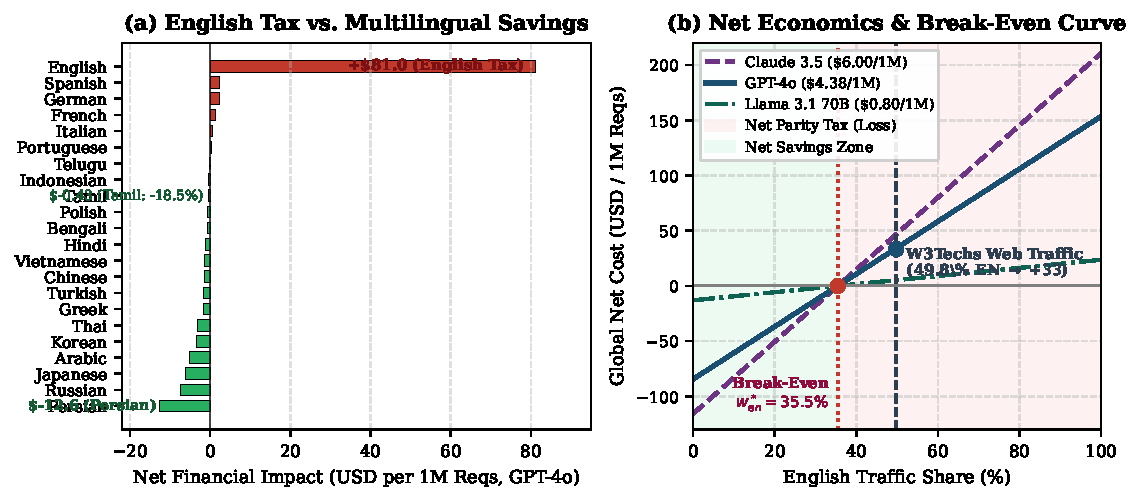
\includegraphics[width=\columnwidth]{figures/fig3_cost_simulation.pdf}
    \vspace{-1.4em}
    \caption{Global financial impact across 1M requests. (a) English Tax ($+\$81.03$) dwarfs non-English savings ($-\$39.87$). (b) Break-even occurs at $w_{\mathrm{en}}^* = 35.5\%$; web ($50\%$) and enterprise ($75\%$) traffic operate in net financial penalty.}
    \label{fig:cost_simulation}
    \vspace{-0.6em}
\end{figure}

{The ``English Tax'' vs.\ Multilingual Savings:} Figure~\ref{fig:cost_simulation}(a) details the financial balance. PA-BPE inflates English token counts by $+8.51\%$ on FLORES-200 ($+35.1$ tokens/req). With English commanding $49.8\%$ of web content, this adds an ``English Tax'' of ${+\$81.03}$ per 1M requests on GPT-4o ($+\$111.12$ on Claude 3.5). While South Asian scripts like Tamil and Telugu save tokens (Tamil: $-18.5\%$; Telugu: $-17.2\%$), their minuscule web share (Tamil: $0.05\%$) caps total savings across all 21 non-English languages at only ${-\$39.87}$. The global net balance is a financial loss of ${+\$41.16}$ per 1M requests on GPT-4o (${+\$56.43}$ on Claude 3.5; ${+\$41,160.00}$ annually per billion requests).

{Break-Even Traffic Dynamics:} In Figure~\ref{fig:cost_simulation}(b), the analytical break-even point occurs at:
\begin{equation}
w_{\mathrm{en}}^* = \frac{-\overline{\Delta T}_{\mathrm{non\text{-}en}}}{\Delta T_{\mathrm{en}} - \overline{\Delta T}_{\mathrm{non\text{-}en}}} = \frac{-(-19.30)}{35.10 - (-19.30)} = {35.48\%}.
\label{eq:breakeven}
\end{equation}
Because web ($50\%$) and enterprise software ($70\%$--$80\%$) exceed $35.5\%$, PA-BPE operates permanently inside the net surcharge zone.

\section{Threats to Validity \& Limitations}
\label{sec:limitations}

{(1) Parametric Reconstruction:} In the absence of public item-level logs in~\cite{foroutan2026parity}, our paired ($\rho=0.60$) and cluster ($\rho_{\mathrm{intra}}=0.25$) models rely on calibrated empirical bounds~\cite{miller2024adding,abadie2022when}; a sensitivity sweep ($\rho \in [0.0, 0.8]$) confirms that downstream differences remain non-significant across the parameter space.
{(2) Merge Scale Invariance:} While trained on scaled corpora, sacrificing tail merges in dominant scripts is an invariant mathematical property of the \textit{fair-max} objective.
{(3) Construct Validity:} Compression parity on general prose ignores token fertility in code, mathematics~\cite{singh2024tokenization}, and commercial APIs~\cite{ahia2023all}.

\section{Conclusion}
\label{sec:conclusion}

Our audit of Parity-Aware BPE yields three findings:
(1) Downstream parity claims lack statistical support; clustering inflates uncertainty by $2.80\times$, rendering all 22 language variations indistinguishable from noise ($p > 0.05$).
(2) Evaluation benchmarks are severely underpowered ($\mathrm{MDE} \pm 9.88\%$), masking severe over-segmentation ($+62\%$ to $+330\%$) in code, arithmetic, and structured JSON.
(3) Under real web traffic, the ``English Tax'' dominates multilingual savings, imposing a net commercial penalty breaking even only when English drops below $35.5\%$.
Cross-lingual fairness requires tokenizer-free byte-level architectures rather than zero-sum vocabulary reallocation.

\section*{AI Assistance Disclosure}
In accordance with course guidelines, the authors declare that Gemini 3.8 (via Antigravity) was used for brainstorming statistical formulas in Python, Matplotlib styling, text enhancing and condensation. All statistical derivations, empirical BPE failure extraction, economic modeling, and analysis were conceived, implemented, and verified by the authors.

\section*{Authorship \& Contribution Statement}

\begin{itemize}
    \item \textbf{Lucas de Oliveira Ferreira (Pessoa 1):}
    Implemented the question-level paired and cross-lingual clustered SE framework (\texttt{paired\_eval.py}); authored Sec.~\ref{sec:stat_methodology}, \ref{sec:results_significance}, and Fig.~\ref{fig:forest_plot}.

    \item \textbf{Mariana Assis Ramos (Pessoa 2):}
    Formulated the Minimum Detectable Effect (MDE) power analysis and executed the reproducible BPE tokenizer failure mode audit (\texttt{power\_and\_failures.py}); authored Sec.~\ref{sec:power_and_failures}, \ref{sec:limitations}, and Table~\ref{tab:failure_modes}.
    
    \item \textbf{João Vitor de Carvalho Silva (Pessoa 3):}
    Led repository setup and Overleaf infrastructure; designed the global API economic simulation and break-even model (\texttt{cost\_simulator.py}); authored Sec.~\ref{sec:intro}, \ref{sec:background}, \ref{sec:financial_impact}, \ref{sec:conclusion}, and Fig.~\ref{fig:cost_simulation}.
\end{itemize}

\bibliographystyle{ACM-Reference-Format}
\bibliography{references}

\end{document}
